\documentclass[1p]{elsarticle_modified}
%\bibliographystyle{elsarticle-num}

%\usepackage[colorlinks]{hyperref}
%\usepackage{abbrmath_seonhwa} %\Abb, \Ascr, \Acal ,\Abf, \Afrak
\usepackage{amsfonts}
\usepackage{amssymb}
\usepackage{amsmath}
\usepackage{amsthm}
\usepackage{scalefnt}
\usepackage{amsbsy}
\usepackage{kotex}
\usepackage{caption}
\usepackage{subfig}
\usepackage{color}
\usepackage{graphicx}
\usepackage{xcolor} %% white, black, red, green, blue, cyan, magenta, yellow
\usepackage{float}
\usepackage{setspace}
\usepackage{hyperref}

\usepackage{tikz}
\usetikzlibrary{arrows}

\usepackage{multirow}
\usepackage{array} % fixed length table
\usepackage{hhline}

%%%%%%%%%%%%%%%%%%%%%
\makeatletter
\renewcommand*\env@matrix[1][\arraystretch]{%
	\edef\arraystretch{#1}%
	\hskip -\arraycolsep
	\let\@ifnextchar\new@ifnextchar
	\array{*\c@MaxMatrixCols c}}
\makeatother %https://tex.stackexchange.com/questions/14071/how-can-i-increase-the-line-spacing-in-a-matrix
%%%%%%%%%%%%%%%

\usepackage[normalem]{ulem}

\newcommand{\msout}[1]{\ifmmode\text{\sout{\ensuremath{#1}}}\else\sout{#1}\fi}
%SOURCE: \msout is \stkout macro in https://tex.stackexchange.com/questions/20609/strikeout-in-math-mode

\newcommand{\cancel}[1]{
	\ifmmode
	{\color{red}\msout{#1}}
	\else
	{\color{red}\sout{#1}}
	\fi
}

\newcommand{\add}[1]{
	{\color{blue}\uwave{#1}}
}

\newcommand{\replace}[2]{
	\ifmmode
	{\color{red}\msout{#1}}{\color{blue}\uwave{#2}}
	\else
	{\color{red}\sout{#1}}{\color{blue}\uwave{#2}}
	\fi
}

\newcommand{\Sol}{\mathcal{S}} %segment
\newcommand{\D}{D} %diagram
\newcommand{\A}{\mathcal{A}} %arc


%%%%%%%%%%%%%%%%%%%%%%%%%%%%%5 test

\def\sl{\operatorname{\textup{SL}}(2,\Cbb)}
\def\psl{\operatorname{\textup{PSL}}(2,\Cbb)}
\def\quan{\mkern 1mu \triangleright \mkern 1mu}

\theoremstyle{definition}
\newtheorem{thm}{Theorem}[section]
\newtheorem{prop}[thm]{Proposition}
\newtheorem{lem}[thm]{Lemma}
\newtheorem{ques}[thm]{Question}
\newtheorem{cor}[thm]{Corollary}
\newtheorem{defn}[thm]{Definition}
\newtheorem{exam}[thm]{Example}
\newtheorem{rmk}[thm]{Remark}
\newtheorem{alg}[thm]{Algorithm}

\newcommand{\I}{\sqrt{-1}}
\begin{document}

%\begin{frontmatter}
%
%\title{Boundary parabolic representations of knots up to 8 crossings}
%
%%% Group authors per affiliation:
%\author{Yunhi Cho} 
%\address{Department of Mathematics, University of Seoul, Seoul, Korea}
%\ead{yhcho@uos.ac.kr}
%
%
%\author{Seonhwa Kim} %\fnref{s_kim}}
%\address{Center for Geometry and Physics, Institute for Basic Science, Pohang, 37673, Korea}
%\ead{ryeona17@ibs.re.kr}
%
%\author{Hyuk Kim}
%\address{Department of Mathematical Sciences, Seoul National University, Seoul 08826, Korea}
%\ead{hyukkim@snu.ac.kr}
%
%\author{Seokbeom Yoon}
%\address{Department of Mathematical Sciences, Seoul National University, Seoul, 08826,  Korea}
%\ead{sbyoon15@snu.ac.kr}
%
%\begin{abstract}
%We find all boundary parabolic representation of knots up to 8 crossings.
%
%\end{abstract}
%\begin{keyword}
%    \MSC[2010] 57M25 
%\end{keyword}
%
%\end{frontmatter}

%\linenumbers
%\tableofcontents
%
\newcommand\colored[1]{\textcolor{white}{\rule[-0.35ex]{0.8em}{1.4ex}}\kern-0.8em\color{red} #1}%
%\newcommand\colored[1]{\textcolor{white}{ #1}\kern-2.17ex	\textcolor{white}{ #1}\kern-1.81ex	\textcolor{white}{ #1}\kern-2.15ex\color{red}#1	}

{\Large $\underline{12a_{1266}~(K12a_{1266})}$}

\setlength{\tabcolsep}{10pt}
\renewcommand{\arraystretch}{1.6}
\vspace{1cm}\begin{tabular}{m{100pt}>{\centering\arraybackslash}m{274pt}}
\multirow{5}{120pt}{
	\centering
	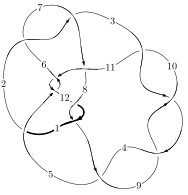
\includegraphics[width=112pt]{../../../GIT/diagram.site/Diagrams/png/2067_12a_1266.png}\\
\ \ \ A knot diagram\footnotemark}&
\allowdisplaybreaks
\textbf{Linearized knot diagam} \\
\cline{2-2}
 &
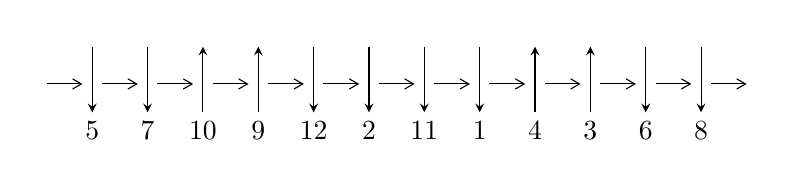
\begin{tikzpicture}[x=20pt, y=17pt]
	% nodes
	\node (C0) at (0, 0) {};
	\node (C1) at (1, 0) {};
	\node (C1U) at (1, +1) {};
	\node (C1D) at (1, -1) {5};

	\node (C2) at (2, 0) {};
	\node (C2U) at (2, +1) {};
	\node (C2D) at (2, -1) {7};

	\node (C3) at (3, 0) {};
	\node (C3U) at (3, +1) {};
	\node (C3D) at (3, -1) {10};

	\node (C4) at (4, 0) {};
	\node (C4U) at (4, +1) {};
	\node (C4D) at (4, -1) {9};

	\node (C5) at (5, 0) {};
	\node (C5U) at (5, +1) {};
	\node (C5D) at (5, -1) {12};

	\node (C6) at (6, 0) {};
	\node (C6U) at (6, +1) {};
	\node (C6D) at (6, -1) {2};

	\node (C7) at (7, 0) {};
	\node (C7U) at (7, +1) {};
	\node (C7D) at (7, -1) {11};

	\node (C8) at (8, 0) {};
	\node (C8U) at (8, +1) {};
	\node (C8D) at (8, -1) {1};

	\node (C9) at (9, 0) {};
	\node (C9U) at (9, +1) {};
	\node (C9D) at (9, -1) {4};

	\node (C10) at (10, 0) {};
	\node (C10U) at (10, +1) {};
	\node (C10D) at (10, -1) {3};

	\node (C11) at (11, 0) {};
	\node (C11U) at (11, +1) {};
	\node (C11D) at (11, -1) {6};

	\node (C12) at (12, 0) {};
	\node (C12U) at (12, +1) {};
	\node (C12D) at (12, -1) {8};
	\node (C13) at (13, 0) {};

	% arrows
	\draw[->,>={angle 60}]
	(C0) edge (C1) (C1) edge (C2) (C2) edge (C3) (C3) edge (C4) (C4) edge (C5) (C5) edge (C6) (C6) edge (C7) (C7) edge (C8) (C8) edge (C9) (C9) edge (C10) (C10) edge (C11) (C11) edge (C12) (C12) edge (C13) ;	\draw[->,>=stealth]
	(C1U) edge (C1D) (C2U) edge (C2D) (C3D) edge (C3U) (C4D) edge (C4U) (C5U) edge (C5D) (C6U) edge (C6D) (C7U) edge (C7D) (C8U) edge (C8D) (C9D) edge (C9U) (C10D) edge (C10U) (C11U) edge (C11D) (C12U) edge (C12D) ;
	\end{tikzpicture} \\
\hhline{~~} \\& 
\textbf{Solving Sequence} \\ \cline{2-2} 
 &
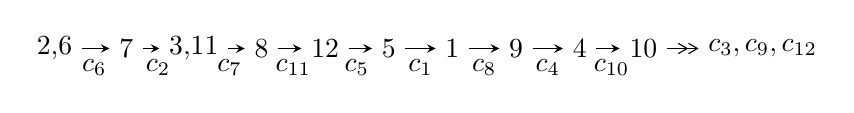
\begin{tikzpicture}[x=23pt, y=7pt]
	% node
	\node (A0) at (-1/8, 0) {2,6};
	\node (A1) at (1, 0) {7};
	\node (A2) at (33/16, 0) {3,11};
	\node (A3) at (25/8, 0) {8};
	\node (A4) at (33/8, 0) {12};
	\node (A5) at (41/8, 0) {5};
	\node (A6) at (49/8, 0) {1};
	\node (A7) at (57/8, 0) {9};
	\node (A8) at (65/8, 0) {4};
	\node (A9) at (73/8, 0) {10};
	\node (C1) at (1/2, -1) {$c_{6}$};
	\node (C2) at (3/2, -1) {$c_{2}$};
	\node (C3) at (21/8, -1) {$c_{7}$};
	\node (C4) at (29/8, -1) {$c_{11}$};
	\node (C5) at (37/8, -1) {$c_{5}$};
	\node (C6) at (45/8, -1) {$c_{1}$};
	\node (C7) at (53/8, -1) {$c_{8}$};
	\node (C8) at (61/8, -1) {$c_{4}$};
	\node (C9) at (69/8, -1) {$c_{10}$};
	\node (A10) at (11, 0) {$c_{3},c_{9},c_{12}$};

	% edge
	\draw[->,>=stealth]	
	(A0) edge (A1) (A1) edge (A2) (A2) edge (A3) (A3) edge (A4) (A4) edge (A5) (A5) edge (A6) (A6) edge (A7) (A7) edge (A8) (A8) edge (A9) ;
	\draw[->>,>={angle 60}]	
	(A9) edge (A10);
\end{tikzpicture} \\ 

\end{tabular} \\

\footnotetext{
The image of knot diagram is generated by the software ``\textbf{Draw programme}" developed by Andrew Bartholomew(\url{http://www.layer8.co.uk/maths/draw/index.htm\#Running-draw}), where we modified some parts for our purpose(\url{https://github.com/CATsTAILs/LinksPainter}).
}\phantom \\ \newline 
\centering \textbf{Ideals for irreducible components\footnotemark of $X_{\text{par}}$} 
 
\begin{align*}
I^u_{1}&=\langle 
2.12438\times10^{16} u^{26}+3.39034\times10^{16} u^{25}+\cdots+3.51214\times10^{17} b-1.86185\times10^{17},\\
\phantom{I^u_{1}}&\phantom{= \langle  }-3.21225\times10^{16} u^{26}+8.75841\times10^{17} u^{25}+\cdots+7.02429\times10^{18} a-4.49004\times10^{18},\;u^{27}- u^{26}+\cdots+9 u+5\rangle \\
I^u_{2}&=\langle 
2.28254\times10^{43} u^{41}-8.69949\times10^{42} u^{40}+\cdots+2.41192\times10^{44} b-1.19984\times10^{44},\\
\phantom{I^u_{2}}&\phantom{= \langle  }-7.56007\times10^{44} u^{41}+5.11353\times10^{44} u^{40}+\cdots+1.20596\times10^{45} a+2.17680\times10^{45},\;u^{42}- u^{41}+\cdots+2 u-1\rangle \\
I^u_{3}&=\langle 
b+u,\;4 a^2-4 a u+2 a- u-2,\;u^2+1\rangle \\
I^u_{4}&=\langle 
b,\;a+1,\;u+1\rangle \\
\\
\end{align*}
\raggedright * 4 irreducible components of $\dim_{\mathbb{C}}=0$, with total 74 representations.\\
\footnotetext{All coefficients of polynomials are rational numbers. But the coefficients are sometimes approximated in decimal forms when there is not enough margin.}
\newpage
\renewcommand{\arraystretch}{1}
\centering \section*{I. $I^u_{1}= \langle 2.12\times10^{16} u^{26}+3.39\times10^{16} u^{25}+\cdots+3.51\times10^{17} b-1.86\times10^{17},\;-3.21\times10^{16} u^{26}+8.76\times10^{17} u^{25}+\cdots+7.02\times10^{18} a-4.49\times10^{18},\;u^{27}- u^{26}+\cdots+9 u+5 \rangle$}
\flushleft \textbf{(i) Arc colorings}\\
\begin{tabular}{m{7pt} m{180pt} m{7pt} m{180pt} }
\flushright $a_{2}=$&$\begin{pmatrix}0\\u\end{pmatrix}$ \\
\flushright $a_{6}=$&$\begin{pmatrix}1\\0\end{pmatrix}$ \\
\flushright $a_{7}=$&$\begin{pmatrix}1\\u^2\end{pmatrix}$ \\
\flushright $a_{3}=$&$\begin{pmatrix}- u\\- u^3+u\end{pmatrix}$ \\
\flushright $a_{11}=$&$\begin{pmatrix}0.00457306 u^{26}-0.124688 u^{25}+\cdots+3.79809 u+0.639216\\-0.0604868 u^{26}-0.0965321 u^{25}+\cdots+1.90841 u+0.530119\end{pmatrix}$ \\
\flushright $a_{8}=$&$\begin{pmatrix}-0.0206853 u^{26}+0.0614281 u^{25}+\cdots+0.192050 u+0.879629\\0.0369043 u^{26}+0.0238101 u^{25}+\cdots-0.476441 u-0.325299\end{pmatrix}$ \\
\flushright $a_{12}=$&$\begin{pmatrix}0.0650598 u^{26}-0.0281555 u^{25}+\cdots+1.88969 u+0.109097\\-0.0604868 u^{26}-0.0965321 u^{25}+\cdots+1.90841 u+0.530119\end{pmatrix}$ \\
\flushright $a_{5}=$&$\begin{pmatrix}0.0140907 u^{26}-0.0116527 u^{25}+\cdots-0.150722 u+0.977059\\0.0259519 u^{26}-0.0340007 u^{25}+\cdots+0.326726 u+0.353353\end{pmatrix}$ \\
\flushright $a_{1}=$&$\begin{pmatrix}0.0243171 u^{26}+0.00525786 u^{25}+\cdots+0.823890 u+0.00567092\\-0.121201 u^{26}-0.108891 u^{25}+\cdots+2.56585 u+0.714641\end{pmatrix}$ \\
\flushright $a_{9}=$&$\begin{pmatrix}0.00888964 u^{26}+0.0799914 u^{25}+\cdots-0.0211326 u+0.758044\\-0.193188 u^{26}+0.0645916 u^{25}+\cdots+1.32901 u+0.280707\end{pmatrix}$ \\
\flushright $a_{4}=$&$\begin{pmatrix}0.0413949 u^{26}-0.0691682 u^{25}+\cdots+0.0713333 u+0.446077\\0.0832991 u^{26}-0.0769045 u^{25}+\cdots-0.735872 u-0.238212\end{pmatrix}$ \\
\flushright $a_{10}=$&$\begin{pmatrix}0.0565987 u^{26}-0.0352749 u^{25}+\cdots+3.17189 u+0.271852\\0.0225032 u^{26}-0.0446485 u^{25}+\cdots+1.00153 u+0.190291\end{pmatrix}$\\&\end{tabular}
\flushleft \textbf{(ii) Obstruction class $= -1$}\\~\\
\flushleft \textbf{(iii) Cusp Shapes $= -\frac{93486209329993615}{351214301166382432} u^{26}+\frac{160253811475151391}{175607150583191216} u^{25}+\cdots-\frac{1621899456495377937}{87803575291595608} u-\frac{3975960787929459125}{351214301166382432}$}\\~\\
\newpage\renewcommand{\arraystretch}{1}
\flushleft \textbf{(iv) u-Polynomials at the component}\newline \\
\begin{tabular}{m{50pt}|m{274pt}}
Crossings & \hspace{64pt}u-Polynomials at each crossing \\
\hline $$\begin{aligned}c_{1},c_{7}\end{aligned}$$&$\begin{aligned}
&16(16 u^{27}+32 u^{26}+\cdots+25 u+11)
\end{aligned}$\\
\hline $$\begin{aligned}c_{2},c_{6},c_{8}\\c_{12}\end{aligned}$$&$\begin{aligned}
&u^{27}- u^{26}+\cdots+9 u+5
\end{aligned}$\\
\hline $$\begin{aligned}c_{3},c_{4},c_{9}\\c_{10}\end{aligned}$$&$\begin{aligned}
&u^{27}+3 u^{26}+\cdots-70 u-10
\end{aligned}$\\
\hline $$\begin{aligned}c_{5},c_{11}\end{aligned}$$&$\begin{aligned}
&u^{27}-3 u^{26}+\cdots+18 u-58
\end{aligned}$\\
\hline
\end{tabular}\\~\\
\newpage\renewcommand{\arraystretch}{1}
\flushleft \textbf{(v) Riley Polynomials at the component}\newline \\
\begin{tabular}{m{50pt}|m{274pt}}
Crossings & \hspace{64pt}Riley Polynomials at each crossing \\
\hline $$\begin{aligned}c_{1},c_{7}\end{aligned}$$&$\begin{aligned}
&256(256 y^{27}-3968 y^{26}+\cdots+977 y-121)
\end{aligned}$\\
\hline $$\begin{aligned}c_{2},c_{6},c_{8}\\c_{12}\end{aligned}$$&$\begin{aligned}
&y^{27}-15 y^{26}+\cdots-59 y-25
\end{aligned}$\\
\hline $$\begin{aligned}c_{3},c_{4},c_{9}\\c_{10}\end{aligned}$$&$\begin{aligned}
&y^{27}+33 y^{26}+\cdots-160 y-100
\end{aligned}$\\
\hline $$\begin{aligned}c_{5},c_{11}\end{aligned}$$&$\begin{aligned}
&y^{27}+15 y^{26}+\cdots-67768 y-3364
\end{aligned}$\\
\hline
\end{tabular}\\~\\
\newpage\flushleft \textbf{(vi) Complex Volumes and Cusp Shapes}
$$\begin{array}{c|c|c}  
\text{Solutions to }I^u_{1}& \I (\text{vol} + \sqrt{-1}CS) & \text{Cusp shape}\\
 \hline 
\begin{aligned}
u &= \phantom{-}0.364874 + 0.825098 I \\
a &= -0.238313 + 0.397025 I \\
b &= \phantom{-}0.112921 - 1.126640 I\end{aligned}
 & \phantom{-}3.64402 - 0.53435 I & \phantom{-}4.34399 + 2.80873 I \\ \hline\begin{aligned}
u &= \phantom{-}0.364874 - 0.825098 I \\
a &= -0.238313 - 0.397025 I \\
b &= \phantom{-}0.112921 + 1.126640 I\end{aligned}
 & \phantom{-}3.64402 + 0.53435 I & \phantom{-}4.34399 - 2.80873 I \\ \hline\begin{aligned}
u &= -1.161210 + 0.177318 I \\
a &= -1.55299 + 0.71207 I \\
b &= -1.02417 + 1.45743 I\end{aligned}
 & -4.02024 + 2.79292 I & -13.1385 - 5.9846 I \\ \hline\begin{aligned}
u &= -1.161210 - 0.177318 I \\
a &= -1.55299 - 0.71207 I \\
b &= -1.02417 - 1.45743 I\end{aligned}
 & -4.02024 - 2.79292 I & -13.1385 + 5.9846 I \\ \hline\begin{aligned}
u &= -1.19546\phantom{ +0.000000I} \\
a &= \phantom{-}1.84775\phantom{ +0.000000I} \\
b &= \phantom{-}1.71581\phantom{ +0.000000I}\end{aligned}
 & -5.68324\phantom{ +0.000000I} & -17.5310\phantom{ +0.000000I} \\ \hline\begin{aligned}
u &= -0.682757 + 0.364207 I \\
a &= \phantom{-}0.789005 - 0.357352 I \\
b &= \phantom{-}0.022604 - 1.395470 I\end{aligned}
 & -0.14501 + 1.44728 I & -5.76179 - 4.68277 I \\ \hline\begin{aligned}
u &= -0.682757 - 0.364207 I \\
a &= \phantom{-}0.789005 + 0.357352 I \\
b &= \phantom{-}0.022604 + 1.395470 I\end{aligned}
 & -0.14501 - 1.44728 I & -5.76179 + 4.68277 I \\ \hline\begin{aligned}
u &= \phantom{-}1.235400 + 0.089712 I \\
a &= \phantom{-}0.774713 - 0.907018 I \\
b &= \phantom{-}0.67807 - 1.77115 I\end{aligned}
 & -13.27050 - 1.98767 I & -16.4839 + 3.0792 I \\ \hline\begin{aligned}
u &= \phantom{-}1.235400 - 0.089712 I \\
a &= \phantom{-}0.774713 + 0.907018 I \\
b &= \phantom{-}0.67807 + 1.77115 I\end{aligned}
 & -13.27050 + 1.98767 I & -16.4839 - 3.0792 I \\ \hline\begin{aligned}
u &= \phantom{-}1.214930 + 0.391524 I \\
a &= \phantom{-}1.60058 + 0.31754 I \\
b &= \phantom{-}0.80643 + 1.29561 I\end{aligned}
 & -2.26047 - 8.25333 I & -7.35249 + 7.59279 I\\
 \hline 
 \end{array}$$\newpage$$\begin{array}{c|c|c}  
\text{Solutions to }I^u_{1}& \I (\text{vol} + \sqrt{-1}CS) & \text{Cusp shape}\\
 \hline 
\begin{aligned}
u &= \phantom{-}1.214930 - 0.391524 I \\
a &= \phantom{-}1.60058 - 0.31754 I \\
b &= \phantom{-}0.80643 - 1.29561 I\end{aligned}
 & -2.26047 + 8.25333 I & -7.35249 - 7.59279 I \\ \hline\begin{aligned}
u &= \phantom{-}1.272470 + 0.241748 I \\
a &= -1.45426 + 0.39776 I \\
b &= -1.380070 + 0.244451 I\end{aligned}
 & -9.23965 - 5.78427 I & -13.7128 + 6.1785 I \\ \hline\begin{aligned}
u &= \phantom{-}1.272470 - 0.241748 I \\
a &= -1.45426 - 0.39776 I \\
b &= -1.380070 - 0.244451 I\end{aligned}
 & -9.23965 + 5.78427 I & -13.7128 - 6.1785 I \\ \hline\begin{aligned}
u &= -0.290377 + 1.268100 I \\
a &= -0.032432 + 0.388759 I \\
b &= -0.230064 - 0.925197 I\end{aligned}
 & \phantom{-}1.90694 - 0.98903 I & -9.51739 + 7.74908 I \\ \hline\begin{aligned}
u &= -0.290377 - 1.268100 I \\
a &= -0.032432 - 0.388759 I \\
b &= -0.230064 + 0.925197 I\end{aligned}
 & \phantom{-}1.90694 + 0.98903 I & -9.51739 - 7.74908 I \\ \hline\begin{aligned}
u &= -1.32694 + 0.50922 I \\
a &= -1.52492 + 0.11633 I \\
b &= -0.70253 + 1.32123 I\end{aligned}
 & -5.85291 + 12.82750 I & -9.51213 - 8.73383 I \\ \hline\begin{aligned}
u &= -1.32694 - 0.50922 I \\
a &= -1.52492 - 0.11633 I \\
b &= -0.70253 - 1.32123 I\end{aligned}
 & -5.85291 - 12.82750 I & -9.51213 + 8.73383 I \\ \hline\begin{aligned}
u &= \phantom{-}0.346727 + 0.443868 I \\
a &= \phantom{-}1.38523 + 1.47579 I \\
b &= \phantom{-}0.249094 + 0.559328 I\end{aligned}
 & -7.24892 - 1.17668 I & -9.05075 + 5.85143 I \\ \hline\begin{aligned}
u &= \phantom{-}0.346727 - 0.443868 I \\
a &= \phantom{-}1.38523 - 1.47579 I \\
b &= \phantom{-}0.249094 - 0.559328 I\end{aligned}
 & -7.24892 + 1.17668 I & -9.05075 - 5.85143 I \\ \hline\begin{aligned}
u &= -1.41709 + 0.38831 I \\
a &= \phantom{-}1.215140 + 0.373473 I \\
b &= \phantom{-}1.248380 + 0.154329 I\end{aligned}
 & -19.0366 + 8.9897 I & -13.6836 - 4.5362 I\\
 \hline 
 \end{array}$$\newpage$$\begin{array}{c|c|c}  
\text{Solutions to }I^u_{1}& \I (\text{vol} + \sqrt{-1}CS) & \text{Cusp shape}\\
 \hline 
\begin{aligned}
u &= -1.41709 - 0.38831 I \\
a &= \phantom{-}1.215140 - 0.373473 I \\
b &= \phantom{-}1.248380 - 0.154329 I\end{aligned}
 & -19.0366 - 8.9897 I & -13.6836 + 4.5362 I \\ \hline\begin{aligned}
u &= \phantom{-}0.31044 + 1.48273 I \\
a &= \phantom{-}0.120252 + 0.379616 I \\
b &= \phantom{-}0.355070 - 0.859580 I\end{aligned}
 & -6.71203 + 1.54503 I & -10.23539 - 4.25212 I \\ \hline\begin{aligned}
u &= \phantom{-}0.31044 - 1.48273 I \\
a &= \phantom{-}0.120252 - 0.379616 I \\
b &= \phantom{-}0.355070 + 0.859580 I\end{aligned}
 & -6.71203 - 1.54503 I & -10.23539 + 4.25212 I \\ \hline\begin{aligned}
u &= \phantom{-}1.41907 + 0.58513 I \\
a &= \phantom{-}1.45781 - 0.00636 I \\
b &= \phantom{-}0.65443 + 1.34532 I\end{aligned}
 & -15.3179 - 15.6052 I & -10.54586 + 7.38863 I \\ \hline\begin{aligned}
u &= \phantom{-}1.41907 - 0.58513 I \\
a &= \phantom{-}1.45781 + 0.00636 I \\
b &= \phantom{-}0.65443 - 1.34532 I\end{aligned}
 & -15.3179 + 15.6052 I & -10.54586 - 7.38863 I \\ \hline\begin{aligned}
u &= -0.187802 + 0.286116 I \\
a &= -0.563690 + 0.885446 I \\
b &= -0.148069 + 0.298333 I\end{aligned}
 & -0.206928 + 0.796519 I & -5.58390 - 8.64848 I \\ \hline\begin{aligned}
u &= -0.187802 - 0.286116 I \\
a &= -0.563690 - 0.885446 I \\
b &= -0.148069 - 0.298333 I\end{aligned}
 & -0.206928 - 0.796519 I & -5.58390 + 8.64848 I\\
 \hline 
 \end{array}$$\newpage\newpage\renewcommand{\arraystretch}{1}
\centering \section*{II. $I^u_{2}= \langle 2.28\times10^{43} u^{41}-8.70\times10^{42} u^{40}+\cdots+2.41\times10^{44} b-1.20\times10^{44},\;-7.56\times10^{44} u^{41}+5.11\times10^{44} u^{40}+\cdots+1.21\times10^{45} a+2.18\times10^{45},\;u^{42}- u^{41}+\cdots+2 u-1 \rangle$}
\flushleft \textbf{(i) Arc colorings}\\
\begin{tabular}{m{7pt} m{180pt} m{7pt} m{180pt} }
\flushright $a_{2}=$&$\begin{pmatrix}0\\u\end{pmatrix}$ \\
\flushright $a_{6}=$&$\begin{pmatrix}1\\0\end{pmatrix}$ \\
\flushright $a_{7}=$&$\begin{pmatrix}1\\u^2\end{pmatrix}$ \\
\flushright $a_{3}=$&$\begin{pmatrix}- u\\- u^3+u\end{pmatrix}$ \\
\flushright $a_{11}=$&$\begin{pmatrix}0.626892 u^{41}-0.424021 u^{40}+\cdots+17.7437 u-1.80503\\-0.0946359 u^{41}+0.0360687 u^{40}+\cdots-2.56626 u+0.497461\end{pmatrix}$ \\
\flushright $a_{8}=$&$\begin{pmatrix}-0.957966 u^{41}+1.20380 u^{40}+\cdots-2.43714 u+0.291897\\0.108267 u^{41}+0.0256008 u^{40}+\cdots+5.44460 u-0.834598\end{pmatrix}$ \\
\flushright $a_{12}=$&$\begin{pmatrix}0.721528 u^{41}-0.460090 u^{40}+\cdots+20.3099 u-2.30250\\-0.0946359 u^{41}+0.0360687 u^{40}+\cdots-2.56626 u+0.497461\end{pmatrix}$ \\
\flushright $a_{5}=$&$\begin{pmatrix}0.620643 u^{41}-0.813885 u^{40}+\cdots+2.26414 u+2.28794\\-0.0198339 u^{41}-0.0132637 u^{40}+\cdots-4.39112 u+0.608259\end{pmatrix}$ \\
\flushright $a_{1}=$&$\begin{pmatrix}2.25050 u^{41}-2.34710 u^{40}+\cdots+11.2525 u-5.46408\\-0.340874 u^{41}+0.341757 u^{40}+\cdots-1.40077 u+0.973676\end{pmatrix}$ \\
\flushright $a_{9}=$&$\begin{pmatrix}0.353819 u^{41}-0.400322 u^{40}+\cdots+5.77072 u-4.35429\\0.197477 u^{41}-0.175445 u^{40}+\cdots-3.35600 u+0.644767\end{pmatrix}$ \\
\flushright $a_{4}=$&$\begin{pmatrix}-0.937637 u^{41}+1.14987 u^{40}+\cdots+13.7232 u+0.948572\\0.307741 u^{41}-0.331030 u^{40}+\cdots-1.73977 u-0.240444\end{pmatrix}$ \\
\flushright $a_{10}=$&$\begin{pmatrix}0.583059 u^{41}-0.427551 u^{40}+\cdots+17.4925 u-1.91785\\-0.121381 u^{41}+0.0565404 u^{40}+\cdots-2.26417 u+0.562919\end{pmatrix}$\\&\end{tabular}
\flushleft \textbf{(ii) Obstruction class $= -1$}\\~\\
\flushleft \textbf{(iii) Cusp Shapes $= 0.351958 u^{41}-0.318899 u^{40}+\cdots+1.24803 u-5.09170$}\\~\\
\newpage\renewcommand{\arraystretch}{1}
\flushleft \textbf{(iv) u-Polynomials at the component}\newline \\
\begin{tabular}{m{50pt}|m{274pt}}
Crossings & \hspace{64pt}u-Polynomials at each crossing \\
\hline $$\begin{aligned}c_{1},c_{7}\end{aligned}$$&$\begin{aligned}
&25(25 u^{42}+85 u^{41}+\cdots+83528 u-95309)
\end{aligned}$\\
\hline $$\begin{aligned}c_{2},c_{6},c_{8}\\c_{12}\end{aligned}$$&$\begin{aligned}
&u^{42}- u^{41}+\cdots+2 u-1
\end{aligned}$\\
\hline $$\begin{aligned}c_{3},c_{4},c_{9}\\c_{10}\end{aligned}$$&$\begin{aligned}
&(u^{21}- u^{20}+\cdots+u+1)^{2}
\end{aligned}$\\
\hline $$\begin{aligned}c_{5},c_{11}\end{aligned}$$&$\begin{aligned}
&(u^{21}+u^{20}+\cdots+u+1)^{2}
\end{aligned}$\\
\hline
\end{tabular}\\~\\
\newpage\renewcommand{\arraystretch}{1}
\flushleft \textbf{(v) Riley Polynomials at the component}\newline \\
\begin{tabular}{m{50pt}|m{274pt}}
Crossings & \hspace{64pt}Riley Polynomials at each crossing \\
\hline $$\begin{aligned}c_{1},c_{7}\end{aligned}$$&$\begin{aligned}
&625(625 y^{42}-15625 y^{41}+\cdots-1.44298\times10^{11} y+9.08381\times10^{9})
\end{aligned}$\\
\hline $$\begin{aligned}c_{2},c_{6},c_{8}\\c_{12}\end{aligned}$$&$\begin{aligned}
&y^{42}-29 y^{41}+\cdots-4 y+1
\end{aligned}$\\
\hline $$\begin{aligned}c_{3},c_{4},c_{9}\\c_{10}\end{aligned}$$&$\begin{aligned}
&(y^{21}+27 y^{20}+\cdots- y-1)^{2}
\end{aligned}$\\
\hline $$\begin{aligned}c_{5},c_{11}\end{aligned}$$&$\begin{aligned}
&(y^{21}+11 y^{20}+\cdots- y-1)^{2}
\end{aligned}$\\
\hline
\end{tabular}\\~\\
\newpage\flushleft \textbf{(vi) Complex Volumes and Cusp Shapes}
$$\begin{array}{c|c|c}  
\text{Solutions to }I^u_{2}& \I (\text{vol} + \sqrt{-1}CS) & \text{Cusp shape}\\
 \hline 
\begin{aligned}
u &= \phantom{-}1.000750 + 0.247732 I \\
a &= \phantom{-}2.15592 - 0.26450 I \\
b &= \phantom{-}0.199725 + 0.739431 I\end{aligned}
 & -2.81557 - 1.02651 I & -5.11271 + 6.49406 I \\ \hline\begin{aligned}
u &= \phantom{-}1.000750 - 0.247732 I \\
a &= \phantom{-}2.15592 + 0.26450 I \\
b &= \phantom{-}0.199725 - 0.739431 I\end{aligned}
 & -2.81557 + 1.02651 I & -5.11271 - 6.49406 I \\ \hline\begin{aligned}
u &= -1.021330 + 0.145152 I \\
a &= \phantom{-}1.56374 - 0.38857 I \\
b &= \phantom{-}0.375476 - 1.140930 I\end{aligned}
 & -0.903078 + 0.771539 I & -5.08724 + 0.81413 I \\ \hline\begin{aligned}
u &= -1.021330 - 0.145152 I \\
a &= \phantom{-}1.56374 + 0.38857 I \\
b &= \phantom{-}0.375476 + 1.140930 I\end{aligned}
 & -0.903078 - 0.771539 I & -5.08724 - 0.81413 I \\ \hline\begin{aligned}
u &= \phantom{-}0.310624 + 1.009640 I \\
a &= -0.212763 - 0.473655 I \\
b &= -0.794642 + 0.241148 I\end{aligned}
 & -13.5849 - 4.1364 I & -11.71281 + 2.17514 I \\ \hline\begin{aligned}
u &= \phantom{-}0.310624 - 1.009640 I \\
a &= -0.212763 + 0.473655 I \\
b &= -0.794642 - 0.241148 I\end{aligned}
 & -13.5849 + 4.1364 I & -11.71281 - 2.17514 I \\ \hline\begin{aligned}
u &= -0.049213 + 1.055370 I \\
a &= \phantom{-}0.152235 - 0.405571 I \\
b &= \phantom{-}0.504141 + 1.153180 I\end{aligned}
 & -1.81098 - 7.30035 I & -6.83891 + 7.23595 I \\ \hline\begin{aligned}
u &= -0.049213 - 1.055370 I \\
a &= \phantom{-}0.152235 + 0.405571 I \\
b &= \phantom{-}0.504141 - 1.153180 I\end{aligned}
 & -1.81098 + 7.30035 I & -6.83891 - 7.23595 I \\ \hline\begin{aligned}
u &= -1.07621\phantom{ +0.000000I} \\
a &= -1.11344\phantom{ +0.000000I} \\
b &= -0.639263\phantom{ +0.000000I}\end{aligned}
 & -1.97351\phantom{ +0.000000I} & -3.86210\phantom{ +0.000000I} \\ \hline\begin{aligned}
u &= \phantom{-}1.100220 + 0.092693 I \\
a &= -1.63403 + 0.13889 I \\
b &= -0.297476 + 1.182770 I\end{aligned}
 & -9.18536 - 0.72644 I & -6.52695 - 0.34896 I\\
 \hline 
 \end{array}$$\newpage$$\begin{array}{c|c|c}  
\text{Solutions to }I^u_{2}& \I (\text{vol} + \sqrt{-1}CS) & \text{Cusp shape}\\
 \hline 
\begin{aligned}
u &= \phantom{-}1.100220 - 0.092693 I \\
a &= -1.63403 - 0.13889 I \\
b &= -0.297476 - 1.182770 I\end{aligned}
 & -9.18536 + 0.72644 I & -6.52695 + 0.34896 I \\ \hline\begin{aligned}
u &= -1.120660 + 0.175896 I \\
a &= -0.46285 + 1.49950 I \\
b &= \phantom{-}0.199725 + 0.739431 I\end{aligned}
 & -2.81557 - 1.02651 I & -5.11271 + 6.49406 I \\ \hline\begin{aligned}
u &= -1.120660 - 0.175896 I \\
a &= -0.46285 - 1.49950 I \\
b &= \phantom{-}0.199725 - 0.739431 I\end{aligned}
 & -2.81557 + 1.02651 I & -5.11271 - 6.49406 I \\ \hline\begin{aligned}
u &= \phantom{-}1.135500 + 0.423437 I \\
a &= -1.41111 - 0.14840 I \\
b &= -0.448707 - 1.150100 I\end{aligned}
 & \phantom{-}1.14110 - 4.04104 I & -1.23432 + 4.27407 I \\ \hline\begin{aligned}
u &= \phantom{-}1.135500 - 0.423437 I \\
a &= -1.41111 + 0.14840 I \\
b &= -0.448707 + 1.150100 I\end{aligned}
 & \phantom{-}1.14110 + 4.04104 I & -1.23432 - 4.27407 I \\ \hline\begin{aligned}
u &= \phantom{-}0.105993 + 0.746952 I \\
a &= \phantom{-}0.184562 - 0.232611 I \\
b &= -0.448707 + 1.150100 I\end{aligned}
 & \phantom{-}1.14110 + 4.04104 I & -1.23432 - 4.27407 I \\ \hline\begin{aligned}
u &= \phantom{-}0.105993 - 0.746952 I \\
a &= \phantom{-}0.184562 + 0.232611 I \\
b &= -0.448707 - 1.150100 I\end{aligned}
 & \phantom{-}1.14110 - 4.04104 I & -1.23432 + 4.27407 I \\ \hline\begin{aligned}
u &= \phantom{-}0.026147 + 1.279880 I \\
a &= -0.282427 - 0.429919 I \\
b &= -0.544516 + 1.163610 I\end{aligned}
 & -10.8630 + 9.1159 I & -8.57432 - 5.67037 I \\ \hline\begin{aligned}
u &= \phantom{-}0.026147 - 1.279880 I \\
a &= -0.282427 + 0.429919 I \\
b &= -0.544516 - 1.163610 I\end{aligned}
 & -10.8630 - 9.1159 I & -8.57432 + 5.67037 I \\ \hline\begin{aligned}
u &= -0.272541 + 0.659489 I \\
a &= -0.013376 - 0.755133 I \\
b &= \phantom{-}0.709616 + 0.181075 I\end{aligned}
 & -4.60791 + 2.71325 I & -10.44742 - 3.99913 I\\
 \hline 
 \end{array}$$\newpage$$\begin{array}{c|c|c}  
\text{Solutions to }I^u_{2}& \I (\text{vol} + \sqrt{-1}CS) & \text{Cusp shape}\\
 \hline 
\begin{aligned}
u &= -0.272541 - 0.659489 I \\
a &= -0.013376 + 0.755133 I \\
b &= \phantom{-}0.709616 - 0.181075 I\end{aligned}
 & -4.60791 - 2.71325 I & -10.44742 + 3.99913 I \\ \hline\begin{aligned}
u &= \phantom{-}1.269690 + 0.210809 I \\
a &= \phantom{-}1.009430 - 0.033264 I \\
b &= \phantom{-}0.709616 - 0.181075 I\end{aligned}
 & -4.60791 - 2.71325 I & -10.44742 + 3.99913 I \\ \hline\begin{aligned}
u &= \phantom{-}1.269690 - 0.210809 I \\
a &= \phantom{-}1.009430 + 0.033264 I \\
b &= \phantom{-}0.709616 + 0.181075 I\end{aligned}
 & -4.60791 + 2.71325 I & -10.44742 - 3.99913 I \\ \hline\begin{aligned}
u &= -1.153270 + 0.592702 I \\
a &= -1.054360 - 0.605877 I \\
b &= -0.515219 + 0.758542 I\end{aligned}
 & -6.73763 + 2.10610 I & -12.68965 - 4.22092 I \\ \hline\begin{aligned}
u &= -1.153270 - 0.592702 I \\
a &= -1.054360 + 0.605877 I \\
b &= -0.515219 - 0.758542 I\end{aligned}
 & -6.73763 - 2.10610 I & -12.68965 + 4.22092 I \\ \hline\begin{aligned}
u &= \phantom{-}1.39064 + 0.33345 I \\
a &= -0.323551 + 0.496463 I \\
b &= -0.515219 + 0.758542 I\end{aligned}
 & -6.73763 + 2.10610 I & -12.68965 + 0. I\phantom{ +0.000000I} \\ \hline\begin{aligned}
u &= \phantom{-}1.39064 - 0.33345 I \\
a &= -0.323551 - 0.496463 I \\
b &= -0.515219 - 0.758542 I\end{aligned}
 & -6.73763 - 2.10610 I & -12.68965 + 0. I\phantom{ +0.000000I} \\ \hline\begin{aligned}
u &= -1.32978 + 0.55644 I \\
a &= \phantom{-}1.224510 - 0.037112 I \\
b &= \phantom{-}0.504141 - 1.153180 I\end{aligned}
 & -1.81098 + 7.30035 I & \phantom{-0.000000 } 0 \\ \hline\begin{aligned}
u &= -1.32978 - 0.55644 I \\
a &= \phantom{-}1.224510 + 0.037112 I \\
b &= \phantom{-}0.504141 + 1.153180 I\end{aligned}
 & -1.81098 - 7.30035 I & \phantom{-0.000000 } 0 \\ \hline\begin{aligned}
u &= -1.46842 + 0.32569 I \\
a &= -0.922519 - 0.020055 I \\
b &= -0.794642 - 0.241148 I\end{aligned}
 & -13.5849 + 4.1364 I & \phantom{-0.000000 } 0\\
 \hline 
 \end{array}$$\newpage$$\begin{array}{c|c|c}  
\text{Solutions to }I^u_{2}& \I (\text{vol} + \sqrt{-1}CS) & \text{Cusp shape}\\
 \hline 
\begin{aligned}
u &= -1.46842 - 0.32569 I \\
a &= -0.922519 + 0.020055 I \\
b &= -0.794642 + 0.241148 I\end{aligned}
 & -13.5849 - 4.1364 I & \phantom{-0.000000 } 0 \\ \hline\begin{aligned}
u &= \phantom{-}1.32647 + 0.78499 I \\
a &= \phantom{-}0.867930 - 0.509797 I \\
b &= \phantom{-}0.631235 + 0.777388 I\end{aligned}
 & -16.2658 - 2.4434 I & \phantom{-0.000000 } 0 \\ \hline\begin{aligned}
u &= \phantom{-}1.32647 - 0.78499 I \\
a &= \phantom{-}0.867930 + 0.509797 I \\
b &= \phantom{-}0.631235 - 0.777388 I\end{aligned}
 & -16.2658 + 2.4434 I & \phantom{-0.000000 } 0 \\ \hline\begin{aligned}
u &= \phantom{-}1.47969 + 0.65675 I \\
a &= -1.114420 + 0.034710 I \\
b &= -0.544516 - 1.163610 I\end{aligned}
 & -10.8630 - 9.1159 I & \phantom{-0.000000 } 0 \\ \hline\begin{aligned}
u &= \phantom{-}1.47969 - 0.65675 I \\
a &= -1.114420 - 0.034710 I \\
b &= -0.544516 + 1.163610 I\end{aligned}
 & -10.8630 + 9.1159 I & \phantom{-0.000000 } 0 \\ \hline\begin{aligned}
u &= -1.58814 + 0.45186 I \\
a &= \phantom{-}0.400910 + 0.274750 I \\
b &= \phantom{-}0.631235 + 0.777388 I\end{aligned}
 & -16.2658 - 2.4434 I & \phantom{-0.000000 } 0 \\ \hline\begin{aligned}
u &= -1.58814 - 0.45186 I \\
a &= \phantom{-}0.400910 - 0.274750 I \\
b &= \phantom{-}0.631235 - 0.777388 I\end{aligned}
 & -16.2658 + 2.4434 I & \phantom{-0.000000 } 0 \\ \hline\begin{aligned}
u &= -0.175560 + 0.250558 I \\
a &= -3.45078 + 4.61056 I \\
b &= -0.297476 - 1.182770 I\end{aligned}
 & -9.18536 + 0.72644 I & -6.52695 + 0.34896 I \\ \hline\begin{aligned}
u &= -0.175560 - 0.250558 I \\
a &= -3.45078 - 4.61056 I \\
b &= -0.297476 + 1.182770 I\end{aligned}
 & -9.18536 - 0.72644 I & -6.52695 - 0.34896 I \\ \hline\begin{aligned}
u &= -0.016547 + 0.283471 I \\
a &= -2.71355 + 0.31034 I \\
b &= \phantom{-}0.375476 + 1.140930 I\end{aligned}
 & -0.903078 - 0.771539 I & -5.08724 - 0.81413 I\\
 \hline 
 \end{array}$$\newpage$$\begin{array}{c|c|c}  
\text{Solutions to }I^u_{2}& \I (\text{vol} + \sqrt{-1}CS) & \text{Cusp shape}\\
 \hline 
\begin{aligned}
u &= -0.016547 - 0.283471 I \\
a &= -2.71355 - 0.31034 I \\
b &= \phantom{-}0.375476 - 1.140930 I\end{aligned}
 & -0.903078 + 0.771539 I & -5.08724 + 0.81413 I \\ \hline\begin{aligned}
u &= \phantom{-}0.175706\phantom{ +0.000000I} \\
a &= \phantom{-}3.58645\phantom{ +0.000000I} \\
b &= -0.639263\phantom{ +0.000000I}\end{aligned}
 & -1.97351\phantom{ +0.000000I} & -3.86210\phantom{ +0.000000I}\\
 \hline 
 \end{array}$$\newpage\newpage\renewcommand{\arraystretch}{1}
\centering \section*{III. $I^u_{3}= \langle b+u,\;4 a^2-4 a u+2 a- u-2,\;u^2+1 \rangle$}
\flushleft \textbf{(i) Arc colorings}\\
\begin{tabular}{m{7pt} m{180pt} m{7pt} m{180pt} }
\flushright $a_{2}=$&$\begin{pmatrix}0\\u\end{pmatrix}$ \\
\flushright $a_{6}=$&$\begin{pmatrix}1\\0\end{pmatrix}$ \\
\flushright $a_{7}=$&$\begin{pmatrix}1\\-1\end{pmatrix}$ \\
\flushright $a_{3}=$&$\begin{pmatrix}- u\\2 u\end{pmatrix}$ \\
\flushright $a_{11}=$&$\begin{pmatrix}a\\- u\end{pmatrix}$ \\
\flushright $a_{8}=$&$\begin{pmatrix}-\frac{1}{2} a+\frac{1}{4} u+\frac{3}{2}\\- a u-2\end{pmatrix}$ \\
\flushright $a_{12}=$&$\begin{pmatrix}a+u\\- u\end{pmatrix}$ \\
\flushright $a_{5}=$&$\begin{pmatrix}a u\\1\end{pmatrix}$ \\
\flushright $a_{1}=$&$\begin{pmatrix}\frac{1}{2} a u+a-\frac{1}{2} u+\frac{1}{4}\\- a+u\end{pmatrix}$ \\
\flushright $a_{9}=$&$\begin{pmatrix}a u- a+\frac{1}{2} u+2\\-2 a u-3\end{pmatrix}$ \\
\flushright $a_{4}=$&$\begin{pmatrix}-3 a u- a+u-\frac{3}{2}\\4 a u+2 a- u+2\end{pmatrix}$ \\
\flushright $a_{10}=$&$\begin{pmatrix}3 a- u\\-4 a+u\end{pmatrix}$\\&\end{tabular}
\flushleft \textbf{(ii) Obstruction class $= 1$}\\~\\
\flushleft \textbf{(iii) Cusp Shapes $= -4$}\\~\\
\newpage\renewcommand{\arraystretch}{1}
\flushleft \textbf{(iv) u-Polynomials at the component}\newline \\
\begin{tabular}{m{50pt}|m{274pt}}
Crossings & \hspace{64pt}u-Polynomials at each crossing \\
\hline $$\begin{aligned}c_{1},c_{7}\end{aligned}$$&$\begin{aligned}
&16(16 u^4+16 u^3+4 u^2+5)
\end{aligned}$\\
\hline $$\begin{aligned}c_{2},c_{5},c_{6}\\c_{8},c_{11},c_{12}\end{aligned}$$&$\begin{aligned}
&(u^2+1)^2
\end{aligned}$\\
\hline $$\begin{aligned}c_{3},c_{4},c_{9}\\c_{10}\end{aligned}$$&$\begin{aligned}
&u^4+3 u^2+1
\end{aligned}$\\
\hline
\end{tabular}\\~\\
\newpage\renewcommand{\arraystretch}{1}
\flushleft \textbf{(v) Riley Polynomials at the component}\newline \\
\begin{tabular}{m{50pt}|m{274pt}}
Crossings & \hspace{64pt}Riley Polynomials at each crossing \\
\hline $$\begin{aligned}c_{1},c_{7}\end{aligned}$$&$\begin{aligned}
&256(256 y^4-128 y^3+176 y^2+40 y+25)
\end{aligned}$\\
\hline $$\begin{aligned}c_{2},c_{5},c_{6}\\c_{8},c_{11},c_{12}\end{aligned}$$&$\begin{aligned}
&(y+1)^4
\end{aligned}$\\
\hline $$\begin{aligned}c_{3},c_{4},c_{9}\\c_{10}\end{aligned}$$&$\begin{aligned}
&(y^2+3 y+1)^2
\end{aligned}$\\
\hline
\end{tabular}\\~\\
\newpage\flushleft \textbf{(vi) Complex Volumes and Cusp Shapes}
$$\begin{array}{c|c|c}  
\text{Solutions to }I^u_{3}& \I (\text{vol} + \sqrt{-1}CS) & \text{Cusp shape}\\
 \hline 
\begin{aligned}
u &= \phantom{-0.000000 -}1.000000 I \\
a &= -0.809017 + 0.500000 I \\
b &= \phantom{-0.000000 } -1.000000 I\end{aligned}
 & -5.59278\phantom{ +0.000000I} & -4.00000\phantom{ +0.000000I} \\ \hline\begin{aligned}
u &= \phantom{-0.000000 -}1.000000 I \\
a &= \phantom{-}0.309017 + 0.500000 I \\
b &= \phantom{-0.000000 } -1.000000 I\end{aligned}
 & \phantom{-}2.30291\phantom{ +0.000000I} & -4.00000\phantom{ +0.000000I} \\ \hline\begin{aligned}
u &= \phantom{-0.000000 } -1.000000 I \\
a &= -0.809017 - 0.500000 I \\
b &= \phantom{-0.000000 -}1.000000 I\end{aligned}
 & -5.59278\phantom{ +0.000000I} & -4.00000\phantom{ +0.000000I} \\ \hline\begin{aligned}
u &= \phantom{-0.000000 } -1.000000 I \\
a &= \phantom{-}0.309017 - 0.500000 I \\
b &= \phantom{-0.000000 -}1.000000 I\end{aligned}
 & \phantom{-}2.30291\phantom{ +0.000000I} & -4.00000\phantom{ +0.000000I}\\
 \hline 
 \end{array}$$\newpage\newpage\renewcommand{\arraystretch}{1}
\centering \section*{IV. $I^u_{4}= \langle b,\;a+1,\;u+1 \rangle$}
\flushleft \textbf{(i) Arc colorings}\\
\begin{tabular}{m{7pt} m{180pt} m{7pt} m{180pt} }
\flushright $a_{2}=$&$\begin{pmatrix}0\\-1\end{pmatrix}$ \\
\flushright $a_{6}=$&$\begin{pmatrix}1\\0\end{pmatrix}$ \\
\flushright $a_{7}=$&$\begin{pmatrix}1\\1\end{pmatrix}$ \\
\flushright $a_{3}=$&$\begin{pmatrix}1\\0\end{pmatrix}$ \\
\flushright $a_{11}=$&$\begin{pmatrix}-1\\0\end{pmatrix}$ \\
\flushright $a_{8}=$&$\begin{pmatrix}0\\1\end{pmatrix}$ \\
\flushright $a_{12}=$&$\begin{pmatrix}-1\\0\end{pmatrix}$ \\
\flushright $a_{5}=$&$\begin{pmatrix}1\\0\end{pmatrix}$ \\
\flushright $a_{1}=$&$\begin{pmatrix}-1\\-1\end{pmatrix}$ \\
\flushright $a_{9}=$&$\begin{pmatrix}-1\\0\end{pmatrix}$ \\
\flushright $a_{4}=$&$\begin{pmatrix}1\\0\end{pmatrix}$ \\
\flushright $a_{10}=$&$\begin{pmatrix}-1\\0\end{pmatrix}$\\&\end{tabular}
\flushleft \textbf{(ii) Obstruction class $= 1$}\\~\\
\flushleft \textbf{(iii) Cusp Shapes $= -12$}\\~\\
\newpage\renewcommand{\arraystretch}{1}
\flushleft \textbf{(iv) u-Polynomials at the component}\newline \\
\begin{tabular}{m{50pt}|m{274pt}}
Crossings & \hspace{64pt}u-Polynomials at each crossing \\
\hline $$\begin{aligned}c_{1},c_{2},c_{7}\\c_{8}\end{aligned}$$&$\begin{aligned}
&u-1
\end{aligned}$\\
\hline $$\begin{aligned}c_{3},c_{4},c_{5}\\c_{9},c_{10},c_{11}\end{aligned}$$&$\begin{aligned}
&u
\end{aligned}$\\
\hline $$\begin{aligned}c_{6},c_{12}\end{aligned}$$&$\begin{aligned}
&u+1
\end{aligned}$\\
\hline
\end{tabular}\\~\\
\newpage\renewcommand{\arraystretch}{1}
\flushleft \textbf{(v) Riley Polynomials at the component}\newline \\
\begin{tabular}{m{50pt}|m{274pt}}
Crossings & \hspace{64pt}Riley Polynomials at each crossing \\
\hline $$\begin{aligned}c_{1},c_{2},c_{6}\\c_{7},c_{8},c_{12}\end{aligned}$$&$\begin{aligned}
&y-1
\end{aligned}$\\
\hline $$\begin{aligned}c_{3},c_{4},c_{5}\\c_{9},c_{10},c_{11}\end{aligned}$$&$\begin{aligned}
&y
\end{aligned}$\\
\hline
\end{tabular}\\~\\
\newpage\flushleft \textbf{(vi) Complex Volumes and Cusp Shapes}
$$\begin{array}{c|c|c}  
\text{Solutions to }I^u_{4}& \I (\text{vol} + \sqrt{-1}CS) & \text{Cusp shape}\\
 \hline 
\begin{aligned}
u &= -1.00000\phantom{ +0.000000I} \\
a &= -1.00000\phantom{ +0.000000I} \\
b &= \phantom{-0.000000 } 0\end{aligned}
 & -3.28987\phantom{ +0.000000I} & -12.0000\phantom{ +0.000000I}\\
 \hline 
 \end{array}$$\newpage
\newpage\renewcommand{\arraystretch}{1}
\centering \section*{ V. u-Polynomials}
\begin{tabular}{m{50pt}|m{274pt}}
Crossings & \hspace{64pt}u-Polynomials at each crossing \\
\hline $$\begin{aligned}c_{1},c_{7}\end{aligned}$$&$\begin{aligned}
&6400(u-1)(16 u^{4}+16 u^{3}+4 u^{2}+5)(16 u^{27}+32 u^{26}+\cdots+25 u+11)\\
&\cdot(25 u^{42}+85 u^{41}+\cdots+83528 u-95309)
\end{aligned}$\\
\hline $$\begin{aligned}c_{2},c_{8}\end{aligned}$$&$\begin{aligned}
&(u-1)(u^2+1)^2(u^{27}- u^{26}+\cdots+9 u+5)(u^{42}- u^{41}+\cdots+2 u-1)
\end{aligned}$\\
\hline $$\begin{aligned}c_{3},c_{4},c_{9}\\c_{10}\end{aligned}$$&$\begin{aligned}
&u(u^4+3 u^2+1)(u^{21}- u^{20}+\cdots+u+1)^{2}(u^{27}+3 u^{26}+\cdots-70 u-10)
\end{aligned}$\\
\hline $$\begin{aligned}c_{5},c_{11}\end{aligned}$$&$\begin{aligned}
&u(u^2+1)^2(u^{21}+u^{20}+\cdots+u+1)^{2}(u^{27}-3 u^{26}+\cdots+18 u-58)
\end{aligned}$\\
\hline $$\begin{aligned}c_{6},c_{12}\end{aligned}$$&$\begin{aligned}
&(u+1)(u^2+1)^2(u^{27}- u^{26}+\cdots+9 u+5)(u^{42}- u^{41}+\cdots+2 u-1)
\end{aligned}$\\
\hline
\end{tabular}\newpage\renewcommand{\arraystretch}{1}
\centering \section*{ VI. Riley Polynomials}
\begin{tabular}{m{50pt}|m{274pt}}
Crossings & \hspace{64pt}Riley Polynomials at each crossing \\
\hline $$\begin{aligned}c_{1},c_{7}\end{aligned}$$&$\begin{aligned}
&40960000(y-1)(256 y^4-128 y^3+176 y^2+40 y+25)\\
&\cdot(256 y^{27}-3968 y^{26}+\cdots+977 y-121)\\
&\cdot(625 y^{42}-15625 y^{41}+\cdots-144297752748 y+9083805481)
\end{aligned}$\\
\hline $$\begin{aligned}c_{2},c_{6},c_{8}\\c_{12}\end{aligned}$$&$\begin{aligned}
&(y-1)(y+1)^4(y^{27}-15 y^{26}+\cdots-59 y-25)\\
&\cdot(y^{42}-29 y^{41}+\cdots-4 y+1)
\end{aligned}$\\
\hline $$\begin{aligned}c_{3},c_{4},c_{9}\\c_{10}\end{aligned}$$&$\begin{aligned}
&y(y^2+3 y+1)^2(y^{21}+27 y^{20}+\cdots- y-1)^{2}\\
&\cdot(y^{27}+33 y^{26}+\cdots-160 y-100)
\end{aligned}$\\
\hline $$\begin{aligned}c_{5},c_{11}\end{aligned}$$&$\begin{aligned}
&y(y+1)^4(y^{21}+11 y^{20}+\cdots- y-1)^{2}\\
&\cdot(y^{27}+15 y^{26}+\cdots-67768 y-3364)
\end{aligned}$\\
\hline
\end{tabular}
\vskip 2pc
\end{document}